\section{Posturographie et signaux posturographiques }

\subsection{Posturographie}

La posturographie, aussi appelée posturologie, est une technique employée pour évaluer, mesurer et contrôler la posture en position debout. 
Pour maintenir un équilibre vertical, le corps humain ajuste en permanence sa posture par rapport à son environnement en fonction de certains signaux qu'il reçoit. 
Ces signaux sont captés par les yeux, la colonne vertébrale, l’oreille interne ou encore les pieds\textsuperscript{\ref{source:1}}. 
Le cerveau les analyse et envoie des instructions au corps dans le but de modifier sa posture en temps réel aux différents éléments perçus. 
Si ces signaux, importants pour le maintien de l'équilibre ne sont pas ou mal perçus, ou mal analysés, la posture ne sera pas correctement adaptée, et des troubles tels que des déséquilibres, des vertiges ou encore des problèmes musculosquelettiques pouvant aller jusqu'à des douleurs chroniques dans certaines régions de l’organisme pourraient apparaître.
Ces études sont possibles aussi bien dans des situations statiques que dynamiques\textsuperscript{\ref{source:2}}.


% \subsubsection{Posturographie dynamique}

La posturographie dynamique informatisée est une technique d'évaluation clinique non invasive\textsuperscript{\ref{source:3}}. 
Cette méthode permet de mesurer et quantifier les mécanismes d’adaptation du système nerveux central intervenant dans le contrôle de la posture et de l'équilibre d’un patient en mouvement. 
Ces mécanismes interviennent aussi bien dans des conditions dites normales (comme pendant des entraînements sportifs), que dans des conditions dites anormales, notamment lors du diagnostic de troubles d'équilibre, de la physiothérapie ou de la rééducation posturale. 
La posturographie dynamique informatisée (CDP) exige différents protocoles\textsuperscript{\ref{source:4}}.


\begin{figure}[H]
  \centering
  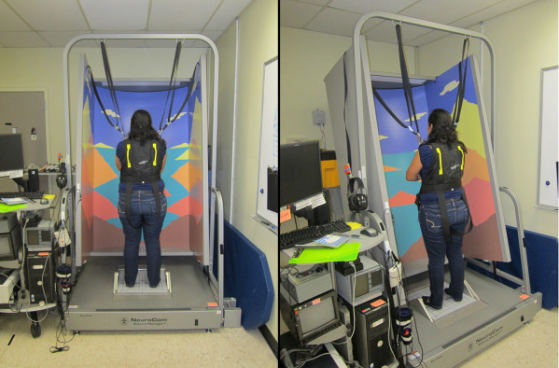
\includegraphics[width=0.5\textwidth]{images/introduction/dynamique.png}
  \caption{Machine d’analyse de la posturographie dynamique }
  \label{fig:posturographie-dynamique}
\end{figure}

% \textbf{Posturographie statique}\\
La posturographie statique évalue, quant à elle, la posture d’un patient en équilibre orthostatique\textsuperscript{\ref{source:5}} (position érigée immobile, fondamentale de l'espèce humaine). 
Cette évaluation se fait en positionnant debout, le patient sur une plateforme équipée de nombreux capteurs de pression. 
L’enregistrement des oscillations du centre de pression des pieds permettent de retracer l'évolution du centre de gravité (ou centre de masse) du patient. 
Lors de ces évaluations, on étudie aussi la réponse posturale du patient à certaines perturbations\textsuperscript{\ref{source:6}}.

\begin{figure}[H]                                                                                                                                                                                                             
  \centering
  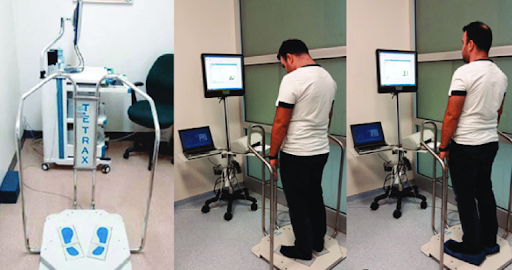
\includegraphics[width=0.5\textwidth]{images/introduction/statique.png}
  \caption{Machine d’analyse de la posturographie statique }
  \label{fig:posturographie-statique}
\end{figure}

\subsection{Signaux Posturographique}

\subsubsection{Types de signaux : pression plantaire}

Les pressions plantaires mesurent la répartition des forces sous les pieds au niveau des zones d’appui. 
Ces pressions sont capturées par des capteurs disposés 
sur une surface ou intégrés dans des semelles. Ces mesures permettent d’identifier les points de pression maximale et minimale, fournissant des données sur la statique et la dynamique du pied.
Les centres de pression sont calculés à partir des variations de pression. 
Ils reflètent les ajustements dynamiques de la posture en réponse aux déséquilibres. 
Les mesures de ces signaux nous permettent de cartographier les zones d'appui et de visualiser les charges appliquées sur les pieds. 
On peut alors identifier les zones à risque de pathologie (comme l’hallux valgus ou la fasciite plantaire)\textsuperscript{\ref{source:7}}. 
L'évaluation des déséquilibres ou anomalies dans la distribution des forces est alors possible. 
Ces études sont appliquées en podologie et orthopédie, pour détecter les troubles plantaires ou les anomalies posturales. 
Elles sont aussi utilisées pour suivre les progrès post-blessures ou post-chirurgie de patients. 
Enfin, on peut aussi les mener dans le but d’optimiser les performances athlétiques en analysant les impacts au sol.

\subsubsection{Examens cliniques}
\label{subsubsec:protocole}

L’équilibre postural d’un patient repose entièrement sur le bon fonctionnement de son système postural. 
De légères perturbations ou dérèglements du fonctionnement de ce système postural peuvent  entraîner un déséquilibre. 
Ainsi, les examens cliniques de l’équilibre statique sont primordiaux pour détecter de potentielles perturbations et éviter par la suite des problèmes de chute. 
Le test classique est le suivant :  le patient est en position debout, fermant les yeux dans des conditions spécifiques.  
L’individu est alors examiné en position debout, talons joints, pieds ouverts à 30°, bras le long du corps. 
Il existe plusieurs autres types de protocoles expérimentaux, dont le Romberg postural\textsuperscript{\ref{source:8}}, le test de piétinement de Fukuda\textsuperscript{\ref{source:9}} ou encore d'autres alternatives.
Une liste de ces protocoles et leur détails est présente en annexe \ref{annexe:1}.

\subsubsection{Enregistrement des signaux}

Les plateformes stabilométriques permettent d'étudier les mouvements posturaux en évaluant les forces verticales et les déplacements dans les plans horizontal et vertical\textsuperscript{\ref{source:10}}. 
Ces plateformes disposent fréquemment d’instruments additionnels, tels que des surfaces instables ou des systèmes de visualisation interactifs, pour perturber l'équilibre et examiner les réactions compensatoires du patient. 
Ces dispositifs sont utilisés pour évaluer la stabilité posturale en position debout, notamment chez des patients atteints de troubles neurologiques ou vestibulaires. 
Ils sont également utilisés pour détecter les déficiences proprioceptives et pour la rééducation.
En gériatrie, ils permettent d'évaluer les risques de chute, et en sport, ils servent à optimiser les stratégies d'équilibre\textsuperscript{\ref{source:11}}. 
\\ \\
Quelques exemples de plateformes stabilométriques existantes : 
\begin{itemize}
    \item Stabilo Stabilometric Platform 
    \item Plateforme  Satel (Figure \ref{fig:satel})
\end{itemize}

\begin{figure}[H]
    \centering
    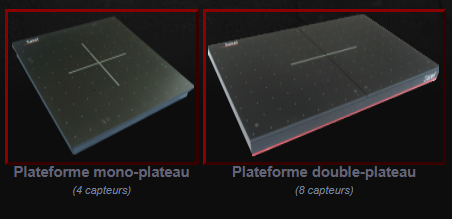
\includegraphics[height=5cm]{images/pression_plantaire/satel.png}
    \caption{Plateforme stabilométrique Satel}\label{fig:satel}
\end{figure}
 
\subsubsection{Méthodes d’analyses}

Pour analyser les signaux posturographiques, des relations mathématiques sont utilisées, permettant de dégager des courbes et des schémas à partir des valeurs numériques. 
Ces relations se basent sur le relevé du centre de pression à l’aide d’une plateforme stabilométrique (figure \ref{fig:satel}) et d’un protocole expérimental (voir [\ref{subsubsec:protocole}]).

Le centre de pression (CdP) reflète les ajustements actifs du corps pour maintenir son équilibre. 
Il est une conséquence des mouvements de ce que l'on appelle le centre de masse (CdM) ou centre de gravité. 

Le CdM est le point théorique correspondant à la position moyenne de la masse corporelle. 
Le corps ajuste constamment la position du CdP afin que les mouvements du CdM ne sortent pas de la surface du support (la zone délimitée par le contact des deux pieds au sol). 
Si le CdM sort de cette surface, le corps ne peut plus maintenir son équilibre et une chute est alors possible.
Ces ajustements engagés par le corps montrent alors que l’accélération du CdM est proportionnelle à la différence entre le CdM et le CdP.

Une relation entre le CdP et le CdM a été modélisée à partir de l’équation mécanique simple du pendule inversé:

\begin{equation}
    CdP = CdM - \frac{h}{g} \times \frac{d^2 CdM}{dt^2} 
    % \label{eq:CdP}
\end{equation}

Cette relation est importante car elle permet d’augmenter la précision des outils mathématiques utilisés pour l’analyse des signaux posturographiques statiques d’un patient. 
Il est à noter que ces outils sont tout de même applicables au CdP.

Les méthodes d'analyse existantes permettent de rendre compte de la qualité ou l'existence des mécanismes de régulation que le corps met en place pour maintenir sa stabilité. 
Il est possible de les analyser aussi bien dans le domaine spatio-temporel que dans le domaine fréquentiel.

L’analyse spatio-temporelle permet de déterminer la qualité de l’équilibre dit orthostatique. 
Elle reflète la capacité du corps d’un patient à maintenir un bon équilibre en position stationnaire droite. 
Dans le domaine spatio-temporel, plusieurs formules sont souvent utilisées pour analyser la qualité de l’équilibre. 
La position moyenne du CdM (voir formules \ref{eq:M_AP} et \ref{eq:M_ML}) permet d’interpréter l’équilibre de manière qualitative. 
La vitesse moyenne du CdM (voir formules \ref{eq:MV_AP} et \ref{eq:MV_ML}) renseigne sur la qualité de l’équilibre ainsi que sur la consommation énergétique du corps pour la régulation de la posture orthostatique. 
Le calcul de la surface de l’ellipse de confiance (CEA) (voir formule \ref{eq:CEA}) décrit l’évolution de l’ellipse de confiance regroupant un certain pourcentage du statokinésigramme. 
Un statokinésigramme est une représentation graphique de la trajectoire du centre de masse, ou bien les déplacements du centre de pression d’un patient. 
D’autres relations sont également couramment utilisées, comme le calcul de l’écart maximal (voir les formules \ref{eq:R_AP} et \ref{eq:R_ML}), la valeur quadratique moyenne (voir les formules \ref{eq:RMS_AP} et \ref{eq:RMS_ML} ou encore le quotient de Romberg (voir \ref{eq:QR}).

Dans le domaine fréquentiel, il est question d’analyse spectrale. 
L’analyse spectrale d’un signal permet d’extraire les différentes composantes présentes dans ce signal et de différencier les nombreux mécanismes utilisés dans le maintien de l’équilibre orthostatique. 
Elle apporte des informations complémentaires à celles obtenues dans le domaine spatio-temporel. 
Le couplage de ces deux types d’analyse permet une meilleure compréhension des mécanismes de maintien de l’équilibre d’un patient. 
Le calcul de la puissance moyenne de la densité spectrale permet de déterminer quelle fréquence domine dans le maintien de l’équilibre du patient. 
Une des méthodes les plus utilisées est l'estimation du périodogramme (voir la section \ref{subsubsec:periodogramme}).
L'estimateur de Welch (formule \ref{eq:P_Welch}) permet d'augmenter la qualité du périodogramme.
L'estimateur du périodogramme et le calcul de l'estimateur de Welch sont des méthodes d'analyse permettant de visualiser la répartition de l'énergie par fréquence.
La fréquence moyenne (ou centroïdale) (voir les formules \ref{eq:FM_AP} et \ref{eq:FM_ML}) permet d’estimer la fréquence centrale des oscillations du corps. 
Cela permet d'estimer le temps nécessaire au mouvement analysé pour revenir dans une position initiale, et permettent de révéler une instabilité (si la fréquence est haute) \textsuperscript{\ref{source:12}}. 
L’analyse de la pente du spectre de puissance (voir section \ref{subsubsec:pente}) permet aussi d’évaluer la stabilité d’un patient.

Les formules et explications pour chacune des méthodes d’analyse décrites ci-dessus sont disponibles en annexe (annexe \ref{annexe:2}).

